% FIRST section - INTRODUCTION 

\section{Introduction}


% The very first letter is a 2 line initial drop letter followed
% by the rest of the first word in caps.
%
% form to use if the first word consists of a single letter:
% \IEEEPARstart{A}{demo} file is ....
%
% form to use if you need the single drop letter followed by
% normal text (unknown if ever used by IEEE):
% \IEEEPARstart{A}{}demo file is ....
%
% Some journals put the first two words in caps:
% \IEEEPARstart{T}{his demo} file is ....
%
% Here we have the typical use of a "T" for an initial drop letter
% and "HIS" in caps to complete the first word.
% \IEEEPARstart{T}{his} demo file is intended to serve as a ``starter file''
% for IEEE journal papers produced under \LaTeX\ using
% IEEEtran.cls version 1.7 and later.
% You must have at least 2 lines in the paragraph with the drop letter
% (should never be an issue)

% Lorem ipsum dolor sit amet, consectetur adipiscing elit, sed do eiusmod tempor incididunt ut labore et dolore magna aliqua. Ut enim ad minim veniam, quis nostrud exercitation ullamco laboris nisi ut aliquip ex ea commodo consequat.  Duis aute irure dolor in reprehenderit in voluptate velit esse cillum dolore eu fugiat nulla pariatur. Excepteur sint occaecat cupidatat non proident, sunt in culpa qui officia deserunt mollit anim id est laborum \cite{Chitambar2019},\cite{CISCO2020}. Excepteur sint occaecat cupidatat non proident, sunt in culpa qui officia deserunt mollit anim id est laborum. See Fig.~\ref{fig:lena1}.

\IEEEPARstart{B}{inaural} audio has been a cornerstone of immersive headphone listening for decades \cite{paul_binaural_2009}. Recently, with its integration into virtual and augmented reality, its popularity has surged significantly \cite{siegfried_binaural_2003}. By exploiting the~human auditory system's perception of sound in natural environments, binaural audio plays a crucial role in creating immersive audio-visual experiences for entertainment applications. Owing to its ability to allow listeners to naturally localize audio sources in direct-to-ear playback, binaural audio has also found successful applications in fields such as avionics \cite{begault_techniques_1992} and hearing aid devices~\cite{thiemann_speech_2016}. The~utility of binaural hearing for these applications is illustrated by the~`cocktail party effect,' which highlights the~human auditory system's ability to focus on foreground sounds while suppressing background noise \cite{cherry_experiments_1953}.

The~increasing availability of binaural audio applications highlights the~need for advanced spatial analysis methods. These methods could facilitate automated, objective assessments of binaural recordings by analyzing spatial characteristics, such as the~position and size of sound sources. Such analysis could support the~development of tools to classify recordings based on these features and help assess the~fidelity of binaural audio systems through spatial characteristics.

The aim of this study is to compare methods for estimating one of the most prominent spatial features: ensemble width. This feature is based on the observation that humans tend to localize groups of sound sources (ensembles) rather than individual sources \cite{bregman_auditory_1990, rumsey_spatial_2002}. The approach draws from Rumsey's scene-based paradigm \cite{rumsey_spatial_2002}, which describes ensemble width as the `overall width of a defined group of sources.' In immersive audio, this feature is particularly important, as wider ensembles enhance the perception of immersion by broadening the spatial distribution of sound sources, creating a more enveloping experience \cite{griesinger_psychoacoustics_1997}. Notably, while one of the presented methods also estimates ensemble location (see Section \ref{sec:methods:neural}), this parameter will be omitted from the study because ensemble width is the only parameter comparable across all three methods.

This paper provides a comparative summary of three ensemble width estimation methods. One of these methods was introduced by Arthi and Sreenivas \cite{arthi_binaural_2022} and later refined by Antoniuk and Zieliński \cite{antoniuk_blind_2023}, while the other two were solely developed by Antoniuk et al. \cite{antoniuk_ensemble_2024, antoniuk_estimating_2024}. The primary contribution of this study is an evaluation of these methods' robustness under more ecologically valid conditions, focusing on their resilience to noise and reverberation. This evaluation offers insights into their applicability in real-world scenarios.

% FIGURE 
% An example of a floating figure using the graphicx package.
% Note that \label must occur AFTER (or within) \caption.
% For figures, \caption should occur after the \includegraphics.
% Note that IEEEtran v1.7 and later has special internal code that
% is designed to preserve the operation of \label within \caption
% even when the captionsoff option is in effect. However, because
% of issues like this, it may be the safest practice to put all your
% \label just after \caption rather than within \caption{}.
%
% Reminder: the "draftcls" or "draftclsnofoot", not "draft", class
% option should be used if it is desired that the figures are to be
% displayed while in draft mode.
%
%\begin{figure}[!t]
%\centering
%\includegraphics[width=2.5in]{myfigure}
% where an .eps filename suffix will be assumed under latex,
% and a .pdf suffix will be assumed for pdflatex; or what has been declared
% via \DeclareGraphicsExtensions.
%\caption{Simulation Results}
%\label{fig_sim}
%\end{figure}

% Note that IEEE typically puts floats only at the top, even when this
% results in a large percentage of a column being occupied by floats.


% An example of a double column floating figure using two subfigures.
% (The subfig.sty package must be loaded for this to work.)
% The subfigure \label commands are set within each subfloat command, the
% \label for the overall figure must come after \caption.
% \hfil must be used as a separator to get equal spacing.
% The subfigure.sty package works much the same way, except \subfigure is
% used instead of \subfloat.
%
%\begin{figure*}[!t]
%\centerline{\subfloat[Case I]\includegraphics[width=2.5in]{subfigcase1}%
%\label{fig_first_case}}
%\hfil
%\subfloat[Case II]{\includegraphics[width=2.5in]{subfigcase2}%
%\label{fig_second_case}}}
%\caption{Simulation results}
%\label{fig_sim}
%\end{figure*}
%
% Note that often IEEE papers with subfigures do not employ subfigure
% captions (using the optional argument to \subfloat), but instead will
% reference/describe all of them (a), (b), etc., within the main caption.

% \begin{figure}[htbp]
% 	\begin{center}
% 		a) 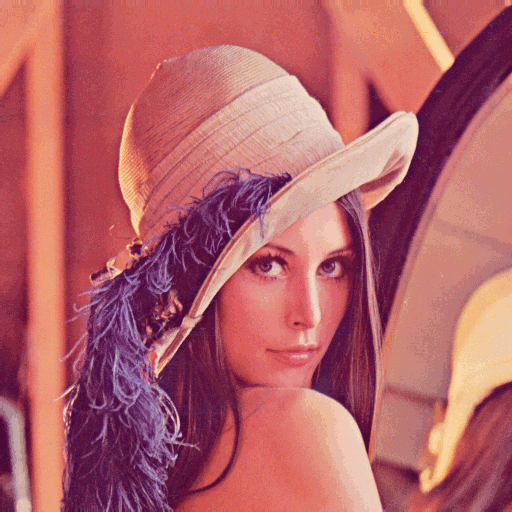
\includegraphics[width=0.4\linewidth]{img/lena.png} 
% 		b) 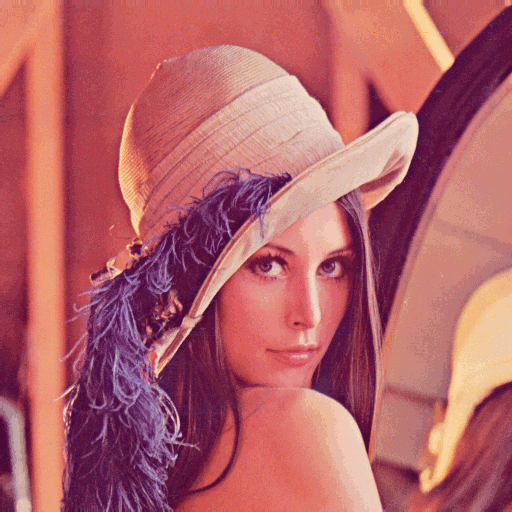
\includegraphics[width=0.4\linewidth]{img/lena.png} 
% 	\end{center}
% 	\caption{Exemplary image of Lena} \label{fig:lena1}
% \end{figure}

% computational coprocessors in classical ICT systems, but so far only for a confined set of problems~\cite{Preskill2018}. Search goes on widening this set.
